\documentclass{article}
\usepackage[utf8]{inputenc}
\usepackage{pgfplots}
\pgfplotsset{width=10cm,compat=1.9}
\usepackage{amsmath,amssymb,amsthm}
\usepackage{graphicx}
\usepackage{float}
\usepackage{blindtext}
\usepackage{hyperref}
\usepackage{verbatim}
\usepackage{gensymb}
\usepackage{enumerate}
\usepackage{xcolor}
\usepackage{graphicx}
\hypersetup{
    colorlinks=true,
    linkcolor=blue,
    filecolor=magenta,      
    urlcolor=cyan,
    pdftitle={Overleaf Example},
    pdfpagemode=FullScreen,
    }
\usepackage[slovene]{babel}

\setlength{\parindent}{0pt}
\setlength{\parskip}{4pt}

\newcounter{example}[section]
\newenvironment{example}[1][]{\refstepcounter{example}\par\medskip
   \noindent \textbf{Naloga~\theexample. #1} \rmfamily}{\medskip}

\newtheorem*{zgled}{Zgled}

\title{Vektorji}
\author{Bor Bregant}
\date{\vspace{-5ex}}

\begin{document}

\thispagestyle{empty}	% ne oštevilči strani

\noindent MATEMATIKA, \quad 2. B \hfill Škofijska klasična gimnazija
\hrule
\vspace{1ex}
\noindent \textbf{Tema:} Opredelitev vektorjev, seštevanje in grafična interpretacija
\vspace{1ex}

\noindent \textbf{Enota:} Vektorji
\vspace{1ex}

\noindent \textbf{Datum:} 24. 10. 2023
\vspace{1ex}

\noindent \textbf{Mentorica:} dr. Marina Rugelj
\vspace{1ex}

\noindent \textbf{Viri in literatura:} Planum novum, 2020, Pavlič G. in drugi
\vspace{1ex}
\hrule
\vspace{2ex}
\noindent \textbf{Učne oblike:} Frontalna, individualna
\vspace{1ex}

\noindent \textbf{Učne metode:} Metoda razprave v uvodu, razlaga
\vspace{1ex}

\noindent \textbf{Učni pripomočki:} Tabla, učbenik
\vspace{1ex}

\noindent \textbf{Učni cilji:} Dijaki/dijakinje narišejo vektorje ter usvojijo seštevanje z vektorji na grafičnem nivoju
\vspace{4ex}
\hrule
\vspace{5ex}
\noindent \textbf{Vsebina in potek:} 

\vspace{5ex}

\section*{\textcolor{violet}{Uvodna motivacija}}

\textbf{\textcolor{violet}{V razpravi poskušamo znanje iz fizike prenesti v matematične vode.}}

Začnemo z uvodom in povezavo s fiziko v razpravi. Primerjamo količine, ki so samo skalarne (npr. temperatura) in količine, ki imajo tudi smer (npr. sila). \textcolor{violet}{Dijaki pri pogovoru sodelujejo.}


\section*{\textcolor{violet}{Razlaga snovi: Opredelitev vektorjev}}

\textbf{\textcolor{violet}{Definicija uvodnih pojmov: Učenci poslušajo in prepišejo v zvezek.}}

Vektor je množica usmerjenih daljic, ki imajo isto velikost in ležijo na vzporednih nosilkah. Operiramo le z enim predstavnikom vektorjev.

Vektorju $\vec{a}=\vec{AB}$ lahko določimo:
\begin{enumerate}[i]
    \item Velikost: $|\vec{AB}|=d(A,B)$,
    \item smer in usmerjenost: Določena s premico nosilko in usmerjenostjo
\end{enumerate}

Vektorja sta enaka, če imata enako velikost, ležita na vzporednih premicah in sta enako usmerjena.

\subsection*{Operacije z vektorji}

\subsubsection*{Seštevanje in odštevanje vektorjev}

Dvočlena operacija, ki dvema vektorjema priredi nov vektor (vsoto). Operacija je komutativna in asociativna.

\begin{enumerate}[i]
    \item Paralelogramsko pravilo,
    \item trikotniško pravilo.
\end{enumerate}

\begin{figure}[H]
    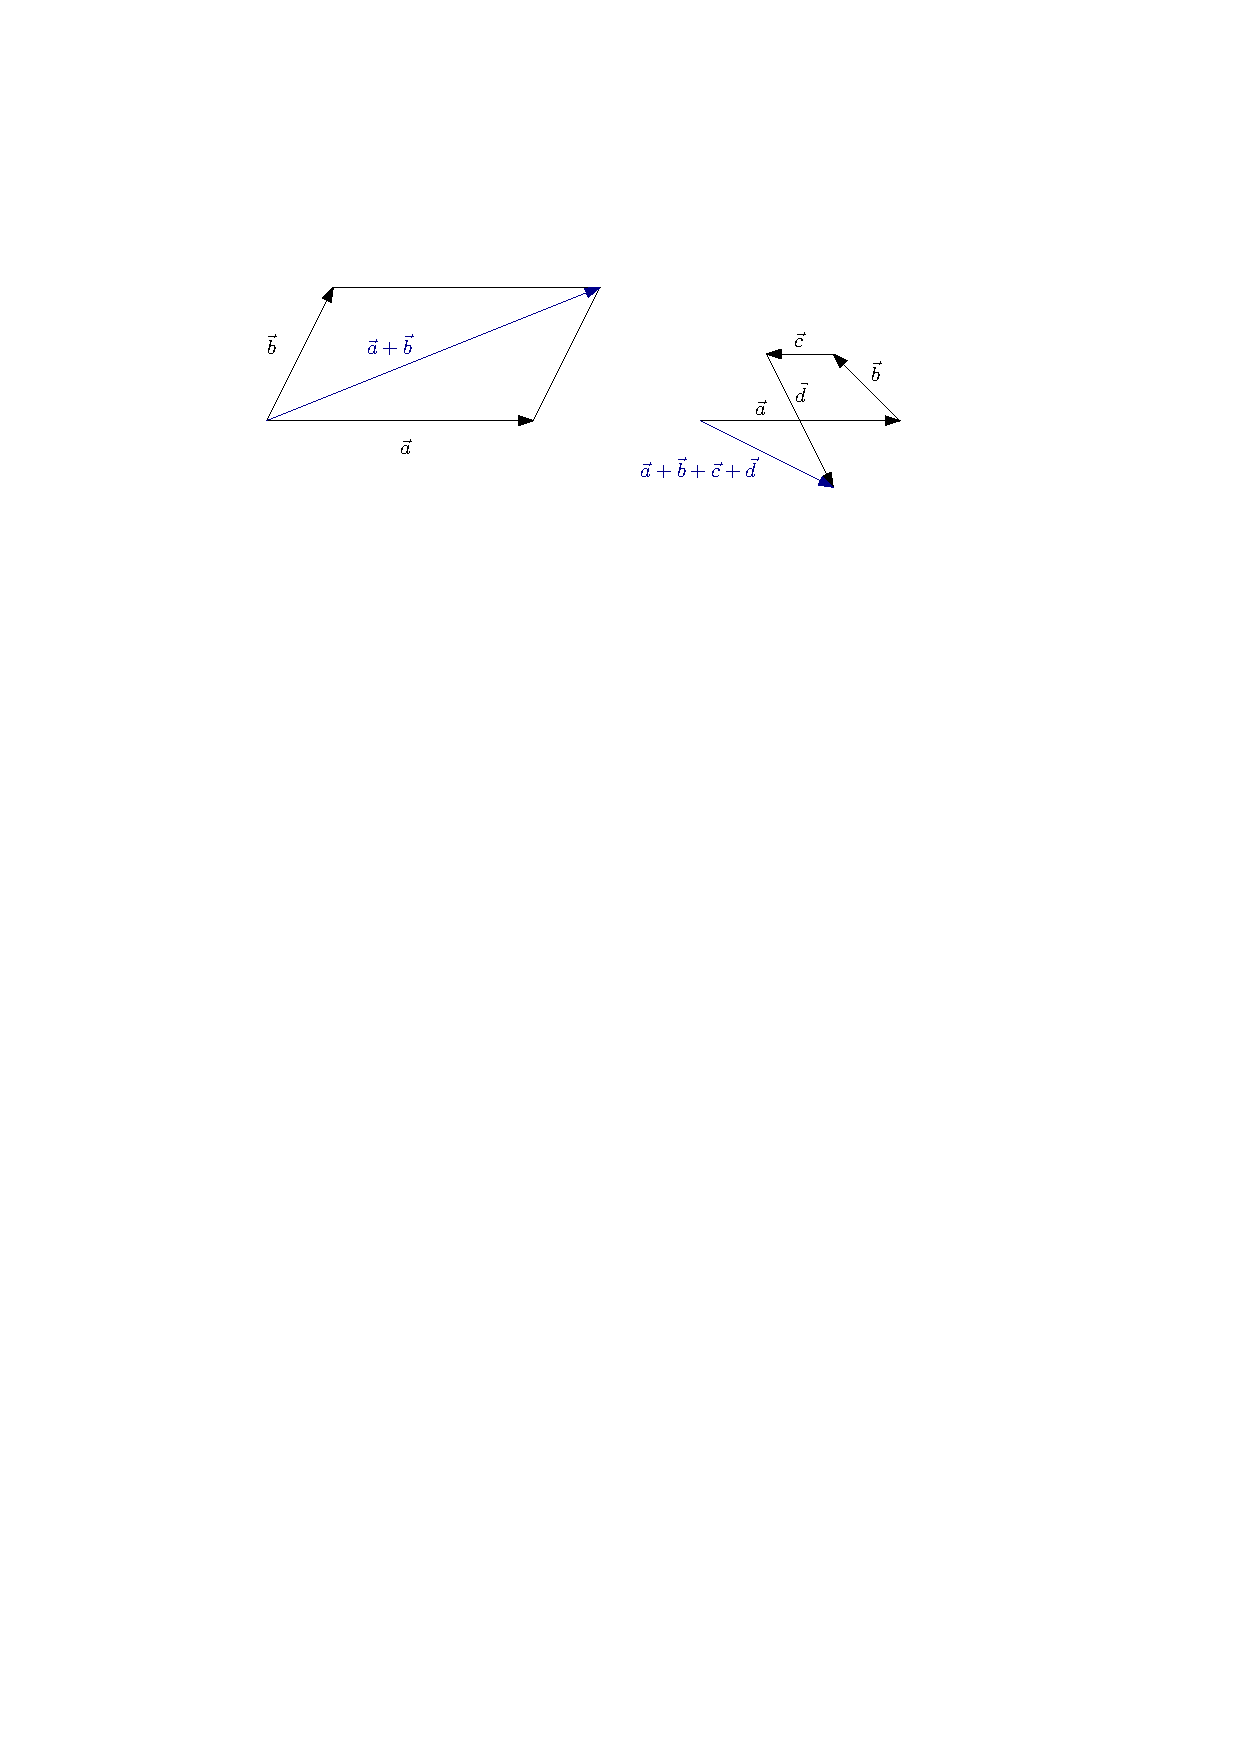
\includegraphics[width=0.7\textwidth]{sestevanje_vektorjev.pdf}
    \centering
\end{figure}

Ničelni vektor $\vec{0}=\vec{AA}=\vec{AB}+\vec{BA}$.

Nasprotni vektor za $\vec{AB}$ je vektor $\vec{BA}$.

Enotski vektor je vektor z dolžino $1$.

Razlika vektorjev  je seštevanje nasprotnega vektorja.

\section*{\textcolor{violet}{Utrjevanje}}
\textbf{\textcolor{violet}{Prvi primer naredimo skupaj, ostale primere pa rešujejo ali pred tablo ali pa individualno (odvisno od klime v razredu).}}



\begin{zgled}
    V pravilnem šestkotniku $ABCDEF$, zapiši vse vektorje, ki so enaki $\vec{AB}$. Zapiši še vse nasprotne vektorje vektorja $\vec{SB}$, kjer je $S$ središče tega šestkotnika.
\end{zgled}

\begin{zgled}
    V kvadratu $ABCD$ izračunaj $\vec{BC}+\vec{CD}$, ter $\vec{DB}-\vec{CB}+\vec{CD}$.
\end{zgled}

\begin{zgled}
    V kocki $ABCDA'B'C'D'$ izračunaj vrednost izrazov $\vec{AD}+\vec{A'B'}$ in $\vec{AB}-\vec{D'A}-\vec{BB'}$.
\end{zgled}

\begin{zgled}
    Izračunaj $\vec{x}$, če je $\vec{x}-\vec{AC}=-\vec{AB}$.
\end{zgled}

\begin{example}
    Domača naloga: 275b, 277bdf,  278e, 281ač, 283c.
\end{example}

\textbf{\textcolor{violet}{Dijaki si DN zabeležijo in odidejo iz razreda}}

\end{document}